\chapter{Algoritmi probabilistici}
Il modello di calcolo di riferimento per gli algoritmi deterministici, inclusi quelli approssimanti visti fin'ora, è quello della macchina di Turing, in cui a un input corrisponde un output (\cref{fig:mdtdet}).
\begin{figure}[ht]
	\centering
	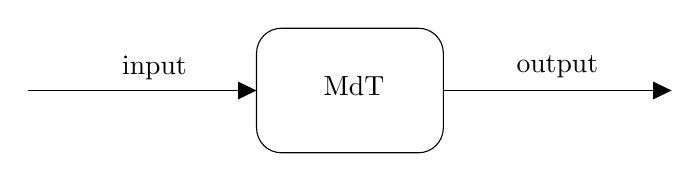
\begin{tikzpicture}[x=0.75pt,y=0.75pt,yscale=-1,xscale=1]
	\draw   (280,152) .. controls (280,145.37) and (285.37,140) .. (292,140) -- (358,140) .. controls (364.63,140) and (370,145.37) .. (370,152) -- (370,188) .. controls (370,194.63) and (364.63,200) .. (358,200) -- (292,200) .. controls (285.37,200) and (280,194.63) .. (280,188) -- cycle ;
	\draw    (170,170) -- (277,170) ;
	\draw [shift={(280,170)}, rotate = 180] [fill={rgb, 255:red, 0; green, 0; blue, 0 }  ][line width=0.08]  [draw opacity=0] (8.93,-4.29) -- (0,0) -- (8.93,4.29) -- cycle    ;
	\draw    (370,170) -- (477,170) ;
	\draw [shift={(480,170)}, rotate = 180] [fill={rgb, 255:red, 0; green, 0; blue, 0 }  ][line width=0.08]  [draw opacity=0] (8.93,-4.29) -- (0,0) -- (8.93,4.29) -- cycle    ;
	\draw (311,162) node [anchor=north west][inner sep=0.75pt]   [align=left] {MdT};
	\draw (214,152) node [anchor=north west][inner sep=0.75pt]   [align=left] {input};
	\draw (404,152) node [anchor=north west][inner sep=0.75pt]   [align=left] {output};
\end{tikzpicture}

	\caption{Macchina di Turing deterministica}
	\label{fig:mdtdet}
\end{figure}

Un diverso modello di calcolo è quello della macchina di Turing probabilistica (\cref{fig:mdtprob}), che ha accesso a una sorgente aleatoria, cioè un input secondario di bit casuali.

\begin{figure}[ht]
	\centering
	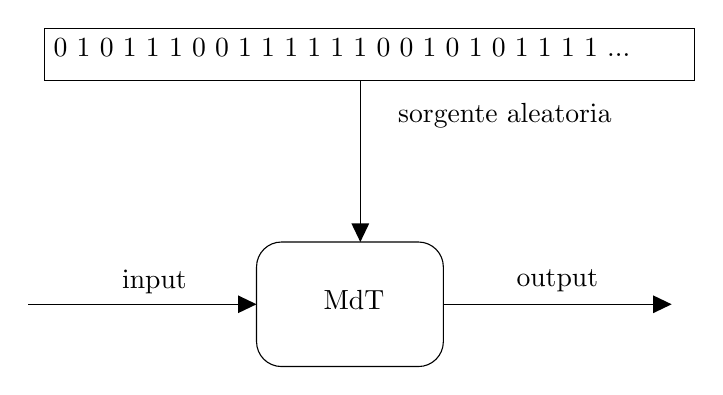
\begin{tikzpicture}[x=0.75pt,y=0.75pt,yscale=-1,xscale=1]
	\draw   (280,152) .. controls (280,145.37) and (285.37,140) .. (292,140) -- (358,140) .. controls (364.63,140) and (370,145.37) .. (370,152) -- (370,188) .. controls (370,194.63) and (364.63,200) .. (358,200) -- (292,200) .. controls (285.37,200) and (280,194.63) .. (280,188) -- cycle ;
	\draw    (170,170) -- (277,170) ;
	\draw [shift={(280,170)}, rotate = 180] [fill={rgb, 255:red, 0; green, 0; blue, 0 }  ][line width=0.08]  [draw opacity=0] (8.93,-4.29) -- (0,0) -- (8.93,4.29) -- cycle    ;
	\draw    (370,170) -- (477,170) ;
	\draw [shift={(480,170)}, rotate = 180] [fill={rgb, 255:red, 0; green, 0; blue, 0 }  ][line width=0.08]  [draw opacity=0] (8.93,-4.29) -- (0,0) -- (8.93,4.29) -- cycle    ;
	\draw    (330,62.29) -- (330,137) ;
	\draw [shift={(330,140)}, rotate = 270] [fill={rgb, 255:red, 0; green, 0; blue, 0 }  ][line width=0.08]  [draw opacity=0] (8.93,-4.29) -- (0,0) -- (8.93,4.29) -- cycle    ;
	\draw (311,162) node [anchor=north west][inner sep=0.75pt]   [align=left] {MdT};
	\draw (214,152) node [anchor=north west][inner sep=0.75pt]   [align=left] {input};
	\draw (404,152) node [anchor=north west][inner sep=0.75pt]   [align=left] {output};
	\draw (347,72) node [anchor=north west][inner sep=0.75pt]   [align=left] {sorgente aleatoria};
	\draw    (178,37) -- (491,37) -- (491,62) -- (178,62) -- cycle  ;
	\draw (181,41) node [anchor=north west][inner sep=0.75pt]   [align=left] { 0 1 0 1 1 1 0 0 1 1 1 1 1 1 0 0 1 0 1 0 1 1 1 1 ...};
\end{tikzpicture}

	\caption{Macchina di Turing probabilistica}
	\label{fig:mdtprob}
\end{figure}

Un algoritmo basato su questo modello si dice probabilistico, in quanto l'output dipende dall'input e dal seme casuale.
L'algoritmo possiede quindi una distribuzione associata, che mappa un input $x$ alla probabilità di ottenere l'output $y$:
\begin{equation*}
	P(Y = y \mid X = x)
\end{equation*}
Gli algoritmi probabilistici possono risolvere problemi di ottimizzazione quanto di decisione e si dividono in due famiglie:
\begin{description}
	\item[Monte Carlo] la correttezza dell'output, cioè la giusta decisione per i problemi di decisione e il calcolo della soluzione ottima per i problemi di ottimizzazione, è probabilistica; il tempo di esecuzione è deterministico;
	\item[Las Vegas] l'output è deterministicamente corretto; il tempo di esecuzione è probabilitico.
\end{description}
È possibile combinare algoritmi approssimanti con algoritmi probabilistici ottenendo algoritmi che approssimano entro una certa soglia dall'ottimo con una certa probabilità.



\section{\MinCut}
\MinCut è il problema di determinare il taglio minimo in un grafo non orientato. In un grafo non orientato $G=(V,E)$, un taglio è dato dalla partizione di $V$ in due sottoinsiemi $X, X\compl$. Il costo del taglio è dato dal numero di archi da vertici in $X$ a vertici in $X\compl$.
\popt{\MinCut}
{$G = (V,E)$}
{Taglio $X\subseteq V$}
{Determinare il taglio minimo in $G$}
{$X\subset V\mid X\neq\emptyset$}
{$\MIN$}
{$\card{\set{e\in E\mid e\cap X\neq\emptyset\land e\setminus X\neq\emptyset}}$}

\noindent\MinCut è un problema \NPO-completo.


\subsection{L'algoritmo di Karger}
L'algoritmo di Karger è un algoritmo Monte Carlo per il taglio minimo e si basa sull'operazione di contrazione.
Sia $G=(V,E)$ un multigrafo\footnote{Nei multigrafi sono ammessi lati paralleli, cioè più lati che incidono sulla stessa coppia di vertici. Consideriamo quindi $E$ un insieme dotato di molteplicità. Formalmente, all'insieme è associata una funzione che indica la molteplicità di ogni elemento. Useremo comunque per semplicità le nozioni insiemistiche per insiemi standard.} di input. Si consideri il multigrafo $G'=(V',E')$, dove:
\begin{itemize}
	\item $V':=\set{\bar v\mid v\in V}$, dove $\bar v:=\set{v}$;
	\item $E':=\set{\set{\bar u,\bar v}\mid \set{u,v}\in E}$.
\end{itemize}
La contrazione $G'\downarrow e$ del lato $e=\set{\bar u,\bar v}$ (\cref{fig:contrazione}) consiste in una modifica di $V'$ e $E'$ come segue:
\begin{enumerate}
	\item viene aggiunto a $V'$ un nuovo supervertice $\bar z=\bar u\cup\bar v$;
	\item ogni arco $\set{\bar u,\bar w}\in E'$, con $w\neq v$, è sostituito da un arco $\set{\bar z,\bar w}$;
	\item ogni arco $\set{\bar w,\bar v}\in E'$, con $w\neq u$, è sostituito da un arco $\set{\bar w,\bar z}$;
	\item gli archi del tipo $\set{\bar u,\bar v}$ vengono rimossi da $E'$;
	\item i vertici $\bar u,\bar v$ vengono rimossi da $V'$.
\end{enumerate}

% TODO: questa immagine andrebbe arricchita un po': non fa capire come si fondono gli archi
\begin{figure}[ht]
	\centering
	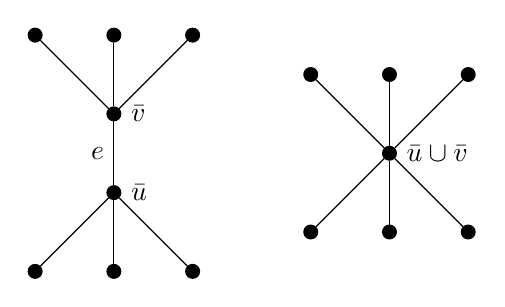
\begin{tikzpicture}[vertex/.style={draw,inner sep=0pt,minimum size=5pt,fill, circle}]
	\node[vertex] at (0, 2)  (u1) {};
	\node[vertex] at (-1, 2)  (u2) {};
	\node[vertex] at (1, 2)  (u3) {};
	\node[vertex,label={0:{$\bar u$}}] at (0, 0)  (a) {};
	\node[vertex,label={0:{$\bar v$}}] at (0, 1)  (b) {};
	\node[vertex] at (0, -1)  (l1) {};
	\node[vertex] at (-1, -1)  (l2) {};
	\node[vertex] at (1, -1)  (l3) {};
	\draw (u1) -- (b);
	\draw (u2) -- (b);
	\draw (u3) -- (b);
	\draw (l1) -- (a);
	\draw (l2) -- (a);
	\draw (l3) -- (a);
	\node at (1.75,0.5) (to) {$\implies$};
	\draw (a) edge node [left] {$e$} (b);
	\node[vertex] at (3.5, 1.5)  (lu1) {};
	\node[vertex] at (2.5, 1.5)  (lu2) {};
	\node[vertex] at (4.5, 1.5)  (lu3) {};
	\node[vertex,label={0:{$\bar u\cup \bar v$}}] at (3.5, 0.5)  (la) {};
	\node[vertex] at (3.5, -0.5)  (ll1) {};
	\node[vertex] at (2.5, -0.5)  (ll2) {};
	\node[vertex] at (4.5, -0.5)  (ll3) {};
	\draw (lu1) -- (la);
	\draw (lu2) -- (la);
	\draw (lu3) -- (la);
	\draw (ll1) -- (la);
	\draw (ll2) -- (la);
	\draw (ll3) -- (la);
\end{tikzpicture}

	\caption{Contrazione $G'\downarrow e$.}
	\label{fig:contrazione}
\end{figure}

In seguito chiameremo semplicemente $G$ il grafo $G'$ derivante dall'input. L'algoritmo \ref{algo:Karger} di Karger effettua contrazioni casuali a partire dal grafo $G$, ottenendo multigrafi $G_0,G_1,\dots$.

\begin{algorithm}[ht]
	\caption{Algoritmo di Karger per \MinCut}
	\label{algo:Karger}
	\SetKwFunction{Unif}{uniformExtraction}
	\SetKwFunction{Connected}{isConnected}
	\SetKwFunction{FindConnected}{findConnectedComponent}
	\SetKwFunction{Choose}{ChooseAnElement}
	\KwInput{grafo $G=(V,E)$}

	\If{$\lnot$\Connected{$G$}}{
		\Return{\FindConnected{$G$}}
	}
	\While{$\card V > 2$}{
		\tcp{Estrai uniformemente a caso un lato e contrailo}
		$e = \Unif{$E$}$

		$G = G\downarrow e$

	}
	\tcp{Restituisci uno dei due vertici rimanenti}
	\Return{\Choose{$V$}}
\end{algorithm}

Chiaramente, l'output dipende dalle scelte dei lati da contrarre, che sono casuali.
Sia $S\star$ il taglio minimo, $k\star$ il numero di lati tagliati da $S\star$ e $G_0,\dots,G_i,\dots$ la sequenza di grafi ottenuti per ogni contrazione operata dall'algoritmo, dove $G_i$ è ottenuto dopo $i$ passi. Si verificano i seguenti fatti:
\begin{oss}\label{oss:kargercontraction}
	\begin{equation*}
		\forall i \quad \card{V_i} = n-i \land \card{E_i} \leq m-i
	\end{equation*}
\end{oss}
\begin{oss}\label{oss:kargercuts}
	Per ogni $i$, ogni taglio in $G_i$ è un taglio in $G$ dello stesso costo.
\end{oss}
\begin{oss}\label{oss:kargermindeg}
	Il grado di ogni vertice di $G_i$ è maggiore o uguale a $k\star$.
\end{oss}

Proviamo ora due lemmi che ci serviranno per dimostrare che l'algoritmo di Karger ottiene la soluzione ottima con buona probabilità.
\begin{lemma}\label{lem:kargeredges}
	\begin{equation*}
		E_i \geq \frac{(n-i) \cdot k\star}{2}
	\end{equation*}
\end{lemma}
\begin{proof}
	\begin{align*}
		\sum_{v\in V_i} d_i(v) \geq \card{V_i} k\star \qquad & \text{per \cref{oss:kargermindeg}}      \\
		\sum_{v\in V_i} d_i(v) \geq (n-i) k\star  \qquad     & \text{per \cref{oss:kargercontraction}} \\
		% TODO: spiegare
		2\card{E_i} \geq (n-i) k\star                                                                  \\
		\card{E_i} \geq \frac{(n-i) k\star}{2}                                                         \\
	\end{align*}
\end{proof}

\begin{lemma}\label{lem:kargerprob_ei}
	Sia $E_i$ l'evento "al passo $i$-esimo (i.e. da $G_i$ a $G_{i+1}$) non viene contratto un lato del taglio minimo". Allora:
	\begin{equation*}
		\forall i \quad P(E_i \mid E_0, \dots, E_{i-1}) \geq \frac{n-i-2}{n-i}
	\end{equation*}
\end{lemma}
\begin{proof}
	\begin{align*}
		P(E_i \mid E_0,\dots,E_{i-1}) & = 1-P(\lnot E_i \mid E_0,\dots,E_{i -1})             \\
		                              & = 1-\frac{k\star}{\card{E_i}}                        \\
		                              & \geq 1-\frac{2k\star}{(n-i)k\star} = 1-\frac{2}{n-i} \\
		                              & = \frac{n-i-2}{n-i}
	\end{align*}
\end{proof}

\begin{theorem}
	L'algoritmo di Karger emette l'ottimo con probabilità $p \geq \frac{1}{{n\choose{2}}}$.
\end{theorem}
\begin{proof}
	L'algoritmo emette l'ottimo se non sono stati contratti archi nel taglio ottimo, ossia se si verifica l'evento $E_0\land E_1\land\dots\land E_{n-3}$. La probabilità di tale evento è
	\begin{align*}
		P(E_0\land E_1\land\dots\land E_{n-3}) & =P(E_0)\cdot P(E_1\mid E_0)\cdots P(E_{n-3}\mid E_0,\dots,E_{n-4})                                              \\
		                                       & \geq\frac{n-2}{n}\cdot\frac{n-3}{n-1}\cdots\frac{n-(n-3)-2}{n-(n-3)} \qquad \text{per \cref{lem:kargerprob_ei}} \\
		                                       & =\frac{n-2}{n}\cdot\frac{n-3}{n-1}\cdots\frac{1}{3}                                                             \\
		                                       & =\frac{(n-2)!}{n!/2}=\frac{2}{n(n-1)}=\frac{1}{\binom{n}{2}}
	\end{align*}
\end{proof}

\begin{corollario}
	Eseguendo l'algoritmo di Karger ${\binom{n}{2}}\ln n$ volte e scegliendo la migliore soluzione si ottiene l'ottimo con probabilità maggiore o uguale a $1-\frac{1}{n}$.
\end{corollario}
\begin{proof}
	Ad ogni esecuzione dell'algoritmo, la probabilità di non trovare l'ottimo è al più
	\begin{equation*}
		1-\frac{1}{\binom{n}{2}}\text.
	\end{equation*}
	Eseguendo l'algoritmo ${\binom{n}{2}}\ln n$ volte, la probabilità che nessun'esecuzione trovi l'ottimo è al più
	\begin{equation*}
		\left(1-\frac{1}{{\binom{n}{2}}}\right)^{{\binom{n}{2}}\ln n}\leq\left(\frac{1}{e}\right)^{\ln n}=\frac{1}{n}\text.
	\end{equation*}
\end{proof}



\section{\MinSetCover}
Si faccia riferimento al paragrafo \ref{sec:SetCover} per la formalizzazione di \MinSetCover.

Il problema può essere trasposto in un problema di programmazione lineare intera di variabili $x_1,\dots,x_m$ e vincoli
\begin{equation*}
	\begin{cases}
		x_j \leq 1                   & \quad \forall j\in m \\
		x_j \geq 0                   & \quad \forall j\in m \\
		\sum_{i:u\in S_i} x_i \geq 1 & \quad \forall u\in U
	\end{cases}
\end{equation*}
Questo problema, in quanto equivalente, ha soluzioni ottime di valore $v\star$ coincidenti con quelle per \MinSetCover.

L'algoritmo probabilistico \ref{algo:ProbRoundingSetCover} risolve polinomialmente all'ottimo il rilassamento continuo $\hat\pi$ di un'istanza così ottenuta, ottenendo una soluzione $\hat x_1,\dots,\hat x_m$ di valore $\hat v\leq v\star$.
Quindi usa i valori $\hat x_i$ come probabilità per scegliere l'insieme $S_i$.
Questa operazione viene ripetuta $\ceil{k+\ln n}$ volte, dove $n:=\card U$ e $k$ è un parametro.

\begin{algorithm}
	\caption{Algoritmo probabilistico basato su arrotondamento per \MinSetCover.}
	\label{algo:ProbRoundingSetCover}
	\KwInput{$S_1,\dots,S_m,w_1,\dots,w_m\in\Q^+,k\in\N^+$}

Sia $\hat\pi$ il problema equivalente di \IntegerLinearProgramming rilassato poi a \LinearProgramming.\;
Siano $\hat x_1,\dots,\hat x_m$ le soluzioni ottime, trovate polinomialmente, per il problema $\hat\pi$.\;
$S\asn\emptyset$\;
\For{$\ceil{k+\log n}$ volte}{
	\For{$i\asn1,\dots,m$}{
		$S\asn S\cup i$ con probabilità $\hat x_i$.\;
	}
}
\Return{$S$}\;

\end{algorithm}

Per l'analisi dell'algoritmo \ref{algo:ProbRoundingSetCover} si richiamano due risultati di probabilità:
\begin{theorem}[disuguaglianza di Markov]\label{thm:markov}
	Per ogni variabile aleatoria $X$ non negativa e per ogni $\beta>0$
	\begin{equation*}
		P[X\geq\beta] \leq \frac{\ev{X}}{\beta}
	\end{equation*}
\end{theorem}
\begin{theorem}[union bound o disuguaglianza di Boole]\label{thm:boole}
	\begin{equation*}
		P\left[\bigcup_i E_i\right] \leq \sum_i P[E_i]
	\end{equation*}
\end{theorem}

\begin{theorem}\label{thm:ammisetcover}
	La probabilità che l'algoritmo \ref{algo:ProbRoundingSetCover} produca una soluzione ammissibile è almeno $1-e^{-k}$.
\end{theorem}
\begin{proof}
	\newcommand{\eve}{\mathcal E}
	La probabilità di trovare una soluzione ammissibile è complementare a quella di non coprire almeno un elemento.
	Chiamiamo $\eve_u$ l'evento dato dalla non copertura dell'elemento $u$.
	La probabilità che l'output sia ammissibile è
	\begin{align*}
		1-P\left[\bigcup_{u\in U} \eve_u\right] & \geq 1-\sum_{u\in U} P[\eve_u]                                     &  & \quad \text{teorema \ref{thm:boole}}                                             \\
		                                        & = 1-\sum_{u\in U}\prod_{i:u\in S_i} P[i\notin I]                   &  & \quad \parbox{5cm}{$u$ non è coperto da nessuno degli insiemi che lo contengono} \\
		                                        & = 1-\sum_{u\in U}\prod_{i:u\in S_i} (1-\hat x_i)^{\ceil{k+\ln n}}                                                                                        \\
		                                        & \geq 1-\sum_{u\in U}\prod_{i:u\in S_i} e^{-\hat x_i\ceil{k+\ln n}} &  & \quad \text{$1-x\leq e^{-x}$}                                                    \\
		                                        & = 1-\sum_{u\in U} e^{-\ceil{k+\ln n}\sum_{i:u\in S_i} \hat x_i}                                                                                          \\
		                                        & \geq \sum_{u\in U} e^{-\ceil{k+\ln n}}                             &  & \quad \text{per vincolo su $\hat x_i$}                                           \\
		                                        & = 1-ne^{-\ceil{k+\ln n}} \geq 1-ne^{-(k+\ln n)}                                                                                                          \\
		                                        & = 1-ne^{-k}e^{-\ln n} = 1-e^{-k} \text.
	\end{align*}
\end{proof}

\begin{theorem}\label{thm:ProbRoundingSetCoveralpha}
	Per ogni $\alpha>0$ e dato $k$, sia $v$ la soluzione prodotta dall'algoritmo \ref{algo:ProbRoundingSetCover}.
	\begin{equation*}
		P\left[\frac{v}{v\star}\geq\alpha(k+\ln n)\right] \leq \frac{1}{\alpha}
	\end{equation*}
\end{theorem}
\begin{proof}
	Calcoliamo il valore atteso di $v$ rispetto all'esecuzione dell'intero algoritmo:
	\begin{align*}
		\ev{v} & = \ev{\sum_{i=1}^m w_i [i\in I]}                                                  \\
		       & = \sum_{i=1}^m w_i \ev{i\in I}                                                    \\
		       & = \sum_{i=1}^m w_i P[i\in I]                                                      \\
		       & \leq \sum_{i=1}^m w_i \hat x_i(k+\ln n) &  & \quad \text{teorema \ref{thm:boole}} \\
		       & = (k+\ln n)\hat v \leq (k+\ln n)v\star
	\end{align*}
	Applicando la disuguaglianza di Markov con $X:=\frac{v}{v\star}$ e $\beta:=\alpha(k+\ln n)$:
	\begin{equation*}
		P\left[\frac{v}{v\star}\geq\alpha(k+\ln n)\right] \leq \frac{\ev{\frac{v}{v\star}}}{\alpha(k+\ln n)} \leq \frac{v\star(k+\ln n)}{v\star}\cdot\frac{1}{\alpha(k+\ln n)}=\frac{1}{\alpha} \text.
	\end{equation*}
\end{proof}

\begin{corollario}
	Eseguendo l'algoritmo \ref{algo:ProbRoundingSetCover} con $k=3$ la probabilità di ottenere una soluzione ammissibile con fattore di approssimazione $\frac{v}{v\star}\leq 6+2\ln n$ è almeno $45\%$.
\end{corollario}
\begin{proof}
	\begin{itemize}
		\item La probabilità che l'algoritmo emetta una soluzione non ammissibile è, in virtù del teorema \ref{thm:ammisetcover}, al più $1-e^{-k}$;
		\item La probabilità che l'algoritmo emetta una soluzione con fattore di approssimazione non inferiore a $6+2\ln n$ è, in virtù del teorema \ref{thm:ammisetcover}, al più $1/2$.
	\end{itemize}

	L'algoritmo emette una soluzione ammissibile e con fattore di approssimazione di al più $6+2\ln n$ complementarmente al produrre una soluzione non ammissibile oppure non buona.
	Pertanto, per union bound, la probabilità di ottenere una soluzione ammissibile e buona è almeno $1-(e^{-3}+\frac12)\geq 45\%$.
\end{proof}



\section{\MaxEkSat}
\MaxEkSat è la versione $k$-indicizzata di \MaxSat: date $t$ clausole
di $k$ letterali ciascuna, l'obiettivo è massimizzare il numero di clausole
soddisfatte.

\popt
{\MaxEkSat}
{Formula booleana nelle variabili $x_1,\dots,x_n$ in forma normale congiuntiva con clausole $c_1,\dots,c_t$ di $k$ letterali senza ripetizione di variabili}
{$\pi:\N\to 2$}
{Determinare il numero massimo di clausole che si possono rendere vere}
{Assegnamenti di valori di verità}
{$\MAX$}
{Numero di clausole rese vere}

\MaxEkSat è \NPO-completo se $k\geq3$.


\subsection{Algoritmo probabilistico}
Un algoritmo probabilistico banale per \MaxEkSat assegna un valore casuale a ogni variabile.
Siano $X_1,\dots,X_n$ variabili aleatorie bernoulliane con probabilità di successo $1/2$.
Sia $T$ la variabile aleatoria corrispondente al numero di clausole rese vere e $C_1,\dots,C_t$ variabili binarie uguali a $1$ se e solo se la clausola relativa è soddisfatta.

\begin{theorem}\label{thm:probassgn}
	Assegnando uniformemente a caso le variabili si ottiene:
	\begin{equation*}
		\ev{T} = \frac{2^k-1}{2^k} t
	\end{equation*}
\end{theorem}
\begin{proof}
	Per la legge del valore atteso totale:
	\begin{align*}
		\ev{T} & = \sum_{b_1\in2}\dots\sum_{b_n\in2} \ev{T\mid X_1=b_1,\dots,X_n=b_n}P[X_1=b_1,\dots,X_n=b_n]                  \\
		       & = \sum_{b_1\in2}\dots\sum_{b_n\in2} \ev{T\mid X_1=b_1,\dots,X_n=b_n}P[X_1=b_1]\cdots P[X_n=b_n]               \\
		       & = \frac{1}{2^n}\sum_{b_1\in2}\dots\sum_{b_n\in2} \ev{T\mid X_1=b_1,\dots,X_n=b_n}                             \\
		       & = \frac{1}{2^n}\sum_{b_1\in2}\dots\sum_{b_n\in2} \ev{C_1+\dots+C_t\mid X_1=b_1,\dots,X_n=b_n}                 \\
		       & = \frac{1}{2^n}\sum_{j=1}^t \left(\sum_{b_1\in2}\dots\sum_{b_n\in2} \ev{C_j\mid X_1=b_1,\dots,X_n=b_n}\right) \\
	\end{align*}
	Il valore atteso di ciascuna variabile $C_j$ dati gli assegnamenti di tutte le variabili è deterministico.
	La loro somma è uguale al numero di assegnamenti che verifica la clausola, cioè il numero di assegnamenti possibili meno quelli che la falsificano, ossia $2^n-2^{n-k}$. Quindi:
	\begin{align*}
		 & = \frac{1}{2^n}\sum_{j=1}^t (2^n-2^{n-k})=\frac{2^n-2^{n-k}}{2^n}t \\
		 & = \frac{2^k-1}{2^k}t
	\end{align*}
\end{proof}

\subsection{Algoritmo derandomizzato}
Il seguente lemma estende il teorema \ref{thm:probassgn} asserendo che il lower bound sul valore atteso può essere preservato se si fissa un determinato assegnamento delle prime $j$ variabili:
\begin{theorem}\label{thm:maxsatderandomexv}
	Per ogni $j=0,\dots,n$ esistono $b_1,\dots,b_j\in2$ tali che
	\begin{equation*}
		\ev{T\mid X_1=b_1,\dots,X_j=b_j} \geq \frac{2^k-1}{2^k}t
	\end{equation*}
\end{theorem}
\begin{proof}
	Per induzione su $j$:
	\begin{itemize}
		\item per $j=0$ la tesi coincide con il teorema \ref{thm:probassgn};
		\item per ipotesi induttiva, per $j$ vale:
		      \begin{equation*}
			      \ev{T\mid X_1=b_1,\dots,X_j=b_j}\geq\frac{2^k-1}{2^k}t \text.
		      \end{equation*}
		      Se per assurdo la tesi fosse falsa in $j+1$, allora varrebbe, sia per $b_{j+1}=0$ sia per $b_{j+1}=1$:
		      \begin{equation}\label{eq:ekpa}
			      \ev{T\mid X_1=b_1,\dots,X_j=b_j,X_{j+1}=b_{j+1}}<\frac{2^k-1}{2^k}t \text.
		      \end{equation}
		      Ma applicando la legge del valore atteso totale all'ipotesi induttiva otteniamo
		      \begin{gather*}
			      \ev{T\mid X_1=b_1,\dots,X_j=b_j} \geq \frac{2^k-1}{2^k}t \\
			      \ev{T\mid X_1=b_1,\dots,X_{j+1}=0}\frac12 + \ev{T\mid X_1=b_1,\dots,X_{j+1}=1}\frac12 \geq \frac{2^k-1}{2^k}t
		      \end{gather*}
		      Che è impossibile se vale (\ref{eq:ekpa}).
	\end{itemize}
\end{proof}

\begin{algorithm}[h]
	\caption{Algoritmo derandomizzato per \MaxEkSat.}
	\label{algo:DerandomMaxEkSat}
	\SetKw{Continue}{continue}

$D \asn \emptyset$
\For{$i\asn1,\dots,n$}{
	$\Delta_0 \asn 0$\;
	$\Delta_1 \asn 0$\;
	$\Delta D_0 \asn \emptyset$\;
	$\Delta D_1 \asn \emptyset$\;
	\For{$j\asn1,\dots,t$}{
		\If{$j\in D$}{
			\Continue\;
		}
		\If {$x_i\notin c_j\land\neg x_i\notin c_j$}{
			\Continue\;
		}
		$h \asn \card{\set{k\mid k>i\land (x_k\in c_j \lor \neg x_k\in c_j)}}$\;
		\If{$\neg x_i\notin c_j$}{
			$\Delta_0 \asn \Delta_0 - \frac{1}{2^h}$\;
			$\Delta_1 \asn \Delta_1 + \frac{1}{2^h}$\;
			$\Delta D_1 \asn \Delta D_1 \cup \{j\}$\;
		}\Else{
			$\Delta_0 \asn \Delta_0 + \frac{1}{2^h}$\;
			$\Delta_1 \asn \Delta_1 - \frac{1}{2^h}$\;
			$\Delta D_0 \asn \Delta D_0 \cup \{j\}$\;
		}
	}
	$u \asn \arg\max_{0,1}(\Delta_0,\Delta_1)$\;
	$X_i \asn u$\;
	$D \asn D \cup \Delta D_u$\;
}

\end{algorithm}

\begin{theorem}
	L'algoritmo \ref{algo:DerandomMaxEkSat} fornisce una $\frac{2^k}{2^k -1}$-approssimazione per \MaxEkSat.
\end{theorem}

% TODO: il teorema va dimostrato. Vanno fatte ulteriori analisi sull'argomento prima di trascrivere quanto detto a lezione, in particolare la formalizzazione va rivista. Non si può parlare di valori attesi in un algoritmo deterministico, e tantomeno si può dare per scontato che gli assegnamenti successivi siano equiprobabili



\section{Il teorema PCP}
Il teorema PCP, \flang{Probabilistically Checkable Proofs}, è uno dei più importanti teoremi della teoria della complessità dal teorema di Cook
Il teorema mette in relazione classi di problemi di decisione riconosciuti da macchine deterministiche con classi riconosciute da macchine con aspetti randomici.


% TODO: decidere se spostare insieme alla definizione di NP nel primo capitolo e includere qui solo i probabilistic checkers
\subsection{Macchine di Turing oracolari}
Le macchine di Turing oracolari sono estensioni delle macchine di Turing che hanno accesso a un oracolo, una stringa $w\in 2\star$ che ha la semantica di certificato.
Una macchina può effettuare una query del bit $w_i$ dell'oracolo inserendo la sua posizione $i$ in un apposito \emph{nastro di query}.
Può poi cambiare stato in funzione del valore del bit restituito.

\begin{figure}[ht]
	\centering
	\begin{tikzpicture}[-arr/.style={-{Latex[scale=1.5]}}]
	\node[draw, rounded corners=5pt,minimum width=2.5cm,minimum height=1.5cm] (tm) {Macchina di Turing};
	\draw[-arr] (-4,0) -- (tm.west)	node[midway,above] {input};
	\draw[-arr] (tm.east) -- (4,0)	node[midway,above] {output};
	\matrix (query) [tape,below=of tm] { 1 & 0 & 1 & 0 & 0 & 1 & 1 & \dots\\};
	\draw[-arr,shorten >=-3.5pt] (tm.south) -- (query.north);
	\node[below=0 of query] {nastro di query};
	\node[draw,rounded corners=3pt,minimum width=1.5cm,minimum height=1cm,right=0.7 of query] (oracolo) {$w$};
	\node[below=0 of oracolo] {oracolo};
	\draw[-arr,shorten <=-3.5pt] (query.east) -- (oracolo.west);
\end{tikzpicture}

	\caption{Macchina di Turing oracolare}
	\label{fig:mdtoracle}
\end{figure}

\begin{defin}
	Un linguaggio $L\subseteq 2^*$ appartiene a $\NP$ se e solo se esiste una macchina di Turing oracolare $V$ tale che:
	\begin{itemize}
		\item $V(x,w)$ termina in un numero di passi polinomiale in $\len x$;
		\item $\forall x\in 2\star \quad \exists w\in 2\star \mid v(x,w)$ accetta $\iff x\in L$.
	\end{itemize}
\end{defin}


\subsection{Verificatori probabilistici}
I verificatori probabilistici (\flang{probabilistic checkers}) estendono ulteriormente le macchine di Turing oracolari potendo accedere a una stringa $r$ di bit casuali giacenti su un apposito nastro.

\begin{figure}[ht]
	\centering
	\begin{tikzpicture}[-arr/.style={-{Latex[scale=1.5]}}]
	\node[draw, rounded corners=5pt,minimum width=2.5cm,minimum height=1.5cm] (tm) {Macchina di Turing};
	\draw[-arr] (-4,0) -- (tm.west)	node[midway,above] {input};
	\draw[-arr] (tm.east) -- (4,0)	node[midway,above] {output};
	\matrix (rand) [tape,above=1 of tm] { 0 & 1 & 0 & 1 & 1 & 1 & 0 & 0 & 1 & 1 & 1 & 1 & 1 & 1 & 0 & 0 & \dots\\};
	\draw[-arr,shorten <=-3.5pt] (rand.south) -- (tm.north);
	\node[above=0 of rand] {sorgente aleatoria};
	\matrix (query) [tape,below=of tm] { 1 & 0 & 1 & 0 & 0 & 1 & 1 & \dots\\};
	\draw[-arr,shorten >=-3.5pt] (tm.south) -- (query.north);
	\node[below=0 of query] {nastro di query};
	\node[draw,rounded corners=3pt,minimum width=1.5cm,minimum height=1cm,right=0.7 of query] (oracolo) {$w$};
	\node[below=0 of oracolo] {oracolo};
	\draw[-arr,shorten <=-3.5pt] (query.east) -- (oracolo.west);
\end{tikzpicture}

	\caption{Verificatore probabilistico}
	\label{fig:probcheck}
\end{figure}

% TODO: approfondire con completeness e soundness? Eventualmente in appendice
I linguaggi binari possono essere classificati in base alle caratteristiche dei verificatori probabilistici che li riconoscono:
\begin{defin}
	Siano $r,q:\N\to\N$ e $L$ un linguaggio.
	$L\in\PCP[r,q]$ se e solo se esiste un verificatore probabilistico $V$ tale che
	\begin{itemize}
		\item $\forall x,R,w$, $V(x,R,w)$ termina in un numero di passi polinomiale in $\len x$;
		\item $\forall x,R,w$, $V(x,R,w)$ effettua al massimo $q(\len x)$ query all'oracolo;
		\item $\forall x,R,w$, $V(x,R,w)$ fa uso di al più $r(\len x)$ bit casuali;
		\item se $x\in L$ allora esiste $w\in 2\star$ tale che $V$ accetta $x$ con probabilità $1$, ossia per ogni stringa casuale $R\in 2^{\leq r(\len x)}$;
		\item se $x\notin L$ allora per qualunque $w$, $V$ rifiuta con probabilità maggiore di $\frac12$, ossia per più di metà delle stringhe casuali $R\in 2^{\leq r(\len x)}$.
	\end{itemize}
	Con abuso di notazione, se $R,Q\subseteq\set{f:\N\to\N}$ allora $\PCP[R,Q]=\bigcup_{r\in R,q\in Q} \PCP[r,q]$.
\end{defin}
\noindent Ad esempio, $\PCP[0,0]=\P$ e, se $\mathrm{Poly}$ è l'insieme delle funzioni al più polinomiali, $\PCP[0,\mathrm{Poly}]=\NP$.

Il teorema PCP limita il nondeterminismo dei verificatori per linguaggi in \NP sostituendolo con un grado di casualità:
\begin{theorem}[PCP \cite{Arora:98:PCP}]\label{thm:pcp}
	$\NP=\PCP[O(\log(n)),O(1)]$.
\end{theorem}


\subsubsection{Verificatori probabilistici normalizzati}
Un verificatore probabilistico è normalizzato se e solo se
\begin{itemize}
	\item estrae tutti i bit casuali all'inizio della computazione;
	\item estratti i bit random effettua tutte le query all'oracolo;
	\item effettuate le query all'oracolo prosegue con il resto della computazione.
\end{itemize}

Si può dimostrare che la classe $\NP=\PCP[O(\log n),O(1)]$ è caratterizzabile unicamente da verificatori probabilistici in forma normale.



\section{Inapprossimabilità}


\subsection{\MaxSat}
\begin{theorem}
	Se $\P\neq\NP$, esiste $\varepsilon>0$ tale che \MaxSat non è $(1+\varepsilon)$-approssimabile in tempo polinomiale.
\end{theorem}
\begin{proof}
	\newcommand{\Rand}{\mathcal R}
	Sia $L$ \NP-completo. Allora per il teorema PCP esistono $\bar q\in O(1)$ e $r\in O(\log n)$ tali che $L\in\PCP[r,q]$.
	Sia $V$ il verificatore probabilistico caratteristico di $L$.
	% TODO: includere approfondimento riguardo al caso in cui il numero di query cambi in base a input e stringa randomica. Quale epsilon si sceglie in quel caso?
	Per semplicità, si assuma che il verificatore effettui esattamente $q\in\N$ query per ogni input e su ogni stringa randomica.
	Il verificatore, ricevuto in input $z\in 2\star$, fa uso di una stringa random $R\in\Rand$ e di un oracolo $w$ su cui effettua al più $q$ query.

	Siano $x^{z,R}_{i_j}$ variabili booleane, dove $i_j$ è la posizione su cui interrogare l'oracolo per la $j$-esima query, con $j\in q$.
	Fissati $z$ ed $R$, il valore di queste variabili è in funzione di $w$, ponendo $x^{z,R}_i:=1\iff w_i=1$.

	Poiché la computazione di $V$ è completamente determinata da $z$, $R$ e $w$, è possibile costruire\footnote{Con una costruzione analoga a quella del teorema di Cook-Levin ciò è possibile in tempo polinomiale.} con le variabili $x^z,R$ una formula booleana $\phi^{z,R}$ che, una volta scelto $w$, abbia valore positivo se e solo se $z$ viene accettato.
	Senza perdita di generalità assumiamo che la formula sia in forma normale congiuntiva e, poiché le variabili sono al più $q$, $\phi^{z,R}$ ha al più $2^q$ clausole con al più $q$ letterali l'una. La dimensione della formula è quindi costante nella lunghezza dell'input.

	Costruiamo una formula $\Phi_z$ che astrae $\phi^{z,R}$ rispetto alla stringa casuale come segue
	\begin{equation*}
		\Phi_z := \bigwedge_{R\in\Rand} \phi^{z,R}
	\end{equation*}
	$\Phi_z$ è in forma normale congiuntiva e, poiché $\Rand$ ha cardinalità logaritmica nella lunghezza dell'input, si può costruire in tempo e spazio polinomiali.

	Fissato $z$, per definizione di verificatore probabilistico uno e uno solo dei seguenti casi si verifica:
	\begin{itemize}
		\item se $z\in L$, esiste un oracolo $w$ per cui $V$ accetta a prescindere dalla stringa casuale $R$. La formula $\Phi_z$ è quindi interamente soddisfacibile usando come assegnamento i valori dei bit di $w$. Il numero di clausole soddisfatte è $\card\Rand 2^q$;
		\item se $z\notin L$, scelto un qualunque oracolo, $V$ accetta con probabilità inferiore a $1/2$, ossia per meno della metà delle stringhe casuali. È possibile soddisfare meno della metà delle sottoformule $\phi^{z,R}$ della formula $\Phi_z$. In termini di clausole, sono soddisfatte $2^q$ clausole per ognuna delle al più $\frac{\card\Rand}{2}$ sottoformule soddisfatte e al più $2^q-1$ per le altre almeno $\frac{\card\Rand}{2}$, per un totale di $\frac{\card\Rand}{2}2^q+\frac{\card\Rand}{2}(2^q-1)$ clausole.
	\end{itemize}

	Sia $\varepsilon:=\frac{1}{2^{q+1}}$.
	Per assurdo, si ammetta che \MaxSat ammetta un algoritmo $\varepsilon$-approssimabile e sia $t$ la soluzione approssimante prodotta da questo algoritmo sull'istanza che consiste nella formula $\Phi_z$.
	Sia $t\star$ la soluzione ottima su tale istanza.
	\begin{itemize}
		\item se $z\in L$ allora
		      \begin{equation*}
			      t \geq \frac{t\star}{1+\varepsilon} = \frac{2^q |\mathcal{R}|}{1+\frac{1}{2^{q+1}}} =: A
		      \end{equation*}
		\item se $z\notin L$ allora
		      \begin{equation*}
			      t \leq t\star < \frac{\card\Rand}{2}2^q+\frac{\card\Rand}{2}(2^q-1) = 2^q\card\Rand-\frac{\card\Rand}{2} =: B
		      \end{equation*}
	\end{itemize}
	Studiando la differenza $A-B$:
	\begin{align*}
		A-B & = \frac{2^q\card\Rand}{1+\frac{1}{2^{q+1}}} - 2^q\card\Rand+\frac{\card\Rand}{2}                           \\
		    & = \card\Rand \frac{2^{q+1} - 2^{q+1}(1+\frac{1}{2^{q+1}}) + (1+\frac{1}{2^{q+1}})}{2(1+\frac{1}{2^{q+1}})} \\
		    & = \card\Rand \frac{2^{q+1} - 2^{q+1}-1 + 1+\frac{1}{2^{q+1}}}{2(1+\frac{1}{2^{q+1}})}                      \\
		    & = \card\Rand \frac{\frac{1}{2^{q+1}}}{2(1 + \frac{1}{2^{q+1}})}                                            \\
		    & > 0 \text.
	\end{align*}

	Poiché $A>B$, è possibile costruire un algoritmo che decida se $z\in L$ in tempo polinomiale come segue:
	\begin{enumerate}
		\item costruire in tempo polinomiale la formula $\Phi_z$ che simula il certificatore $V$;
		\item eseguire l'algoritmo polinomiale che $1+\varepsilon$-approssima \MaxSat su $\Phi_z$, ottenendo una soluzione di valore $t$;
		\item se $t\geq A$ allora $z\in L$; se $t\leq B$ allora $z\notin L$.
		      Poiché $L$ è \NP-completo, ciò è impossibile se $\P\neq\NP$.
	\end{enumerate}
\end{proof}


\subsection{\IndependentSet}
Il problema dell'insieme indipendente consiste nel determinare l'insieme indipendente di cardinalità massima in un dato grafo.
Dato un grafo $G=(V,E)$, un insieme indipendente è un insieme $X\subseteq V$ che non contiene vertici a due a due adiacenti, ossia tale che $\forall i,j\in X:\set{i,j}\notin E$.

\popt{\IndependentSet}
{Grafo $G=(V,E)$}
{$X\subseteq V$}
{Determinare l'insieme indipendente di cardinalità massima in $G$}
{$X$ è un insieme indipendente}
{$\MAX$}
{$\card X$}

Grazie al teorema PCP si può limitare l'approssimabilità di \IndependentSet a non meno di $2$:
\begin{theorem}\label{thm:ind_set_inapprox}
	Se $\P\neq\NP$ allora, per ogni $\varepsilon>0$, \IndependentSet non è $(2-\varepsilon)$-approssimabile in tempo polinomiale.
\end{theorem}
\begin{proof}
	Sia $L$ \NP-completo. Allora per il teorema PCP esistono $q\in O(1)$ e $r\in O(\log n)$ tali che $L\in\PCP[r,q]$.
	Sia $V$ il verificatore probabilistico caratteristico di $L$.

	Fissato un input $z$ accettato da $V$, si dice configurazione di $V$ una tupla $C:=\tuple{R,I,f}$ composta da:
	\begin{itemize}
		\item una stringa $R\in 2^{r(\len z)}$ di bit random;
		\item un insieme $I\subseteq\N$ di indici di posizioni dell'oracolo di cui effettuare query, di cardinalità al più $\card I=q(\len z)$;
		\item una funzione $f:I\to 2$ che restituisce il valore di ogni query all'oracolo.
	\end{itemize}
	Due configurazioni $C_1$ e $C_2$ si dicono compatibili se e solo se si verificano le due seguenti condizioni
	\begin{itemize}
		\item $R_{C_1}\neq R_{C_2}$;
		\item $\forall i\in I_{C_1}\cap I_{C_2},\quad f_{C_1}(i)=f_{C_2}(i)$.
	\end{itemize}

	Fissato $z$, sia $G$ un grafo non orientato in cui i vertici sono le configurazioni di $V$ e due vertici sono adiacenti se e solo se le rispettive configurazioni sono incompatibili (cioè non compatibili).
	Il grafo si può costruire in tempo polinomiale in $\len z$ essendo il numero dei suoi vertici nell'ordine di $2^{r(\len z)}\cdot 2^q$.

	\begin{fact}\label{fac:indip1}
		Se $z\in L$, $G$ ha un insieme indipendente di cardinalità maggiore o uguale a $2^{r(\len z)}$.
	\end{fact}
	\begin{proof}
		Se $z\in L$, per definizione di verificatore probabilistico esiste un certificato $w$ tale per cui $V$ accetta su ogni stringa casuale.
		Tutte le configurazioni $C$ di $V$ con query compatibili con $w$, ossia tali che $f_C(i)=w_i\forall i\in I_C$ e che spaziano su tutti i valori $R_C\in 2^{r(\len z)}$, sono tra loro compatibili, quindi i rispettivi vertici danno luogo a un insieme indipendente.
		Questi sono nel numero delle stringhe casuali, cioè $2^{r(\len z)}$.
	\end{proof}

	\begin{fact}\label{fac:indip2}
		Se $z\notin L$, ogni insieme indipendente di $G$ ha cardinalità minore di $\frac{2^{r(\len z)}}{2}$.
	\end{fact}
	\begin{proof}
		Per assurdo, si ammetta l'esistenza di un insieme indipendente $X$ con cardinalità di almeno $\frac{2^{r(\len z)}}{2}$.
		I vertici in tale insieme corrispondono a configurazioni con diverse sequenze di bit randomici e con query non discordanti.
		Si può quindi costruire una stringa $w$ compatibile con tutte le query di ogni configurazione, cioè tale per cui per ogni configurazione $C\in X$, $f_C(i)=w_i\forall i\in I_C$.
		Poiché la stringa è un oracolo accettante per più di $\frac{2^{r(\len z)}}{2}$ stringhe casuali, la macchina accetta con probabilità di almeno $\frac12$, il che è impossibile se $z\notin L$.
	\end{proof}

	Per assurdo, sia $A$ un algoritmo $2-\varepsilon$-approssimante per \IndependentSet.
	\begin{itemize}
		\item Se $z\in L$ allora in virtù del fatto \ref{fac:indip1} l'algoritmo emette un output dal valore di almeno $\frac{2^{r(\len z)}}{2-\varepsilon}>\frac{2^{r(\len z)}}{2}$;
		\item se $z\notin L$ allora in virtù del fatto \ref{fac:indip2} l'algoritmo emette un output di valore minore di $\frac{2^{r(\len z)}}{2}$.
	\end{itemize}
	L'algoritmo potrebbe quindi decidere in tempo polinomiale il linguaggio $L$, il che è impossibile se $\P\neq\NP$.
\end{proof}
